\documentclass{IMTexam}

\usepackage[enums]{IMTtikz}

\givecredits
\author{Isabella B. Amaral}
\USPN{118010773}
\lecture{Matemática I}
\examname{Prova II}
\hwtype{Resolução}
\lcode{}
\date{4 de novembro}

\newtheorem{theorem}{Teorema}[question]
\newtheorem{corollary}{Corolário}[theorem]
\newtheorem{lemma}[theorem]{Lema}
\let\oldemptyset\emptyset
\let\emptyset\varnothing
\usepackage{mathtools}
\DeclarePairedDelimiter\ceil{\lceil}{\rceil}
\DeclarePairedDelimiter\floor{\lfloor}{\rfloor}


\begin{document}
	
	\maketitle
	
	\paragraph{Nota:} Todos os teoremas e axiomas referenciados nessa prova são citados pelo Apostol nos dois primeiros capítulos do livro de cálculo I, a não ser que seja explicitado o contrário.
	
	\paragraph{Nota 2:} As resoluções dessa prova foram fortemente inspiradas por colegas, por conta da dinâmica adotada na resolução.
	
	\begin{questions}
		\question Calcular a área entre os gráficos de $ f(x) = \sin x, 0 \leqslant x \leqslant \pi $ e $ g(x) = 2x(x − \pi), 0 \leqslant x \leqslant \pi $.
		
		\begin{solution}
			Sabemos que para $ 0\leqslant x \leqslant \pi $, $ \sin x\geqslant 0 $ e $ 2x(x-\pi)\leqslant 0 $, por uma simples análise gráfica, e que as únicas intercessões entre as funções se dão para $ x=0 $ e $ x=\pi $, então podemos integrar a região entre elas simplesmente fazendo
			\begin{align*}
				&\int_{0}^{\pi}\sin x - 2x(x-\pi)\dif x\\ \intertext{pela propriedade aditiva}
				\iff &\int_{0}^{\pi}\sin x \dif x - \int_{0}^{\pi} 2x^{2}\dif x +\int_{0}^{\pi}2x\,\pi\dif x\\
				\implies &\eval{\del{-\cos x}}_{0}^{\pi} - \eval{\dfrac{2}{3}x^{3}}_{0}^{\pi} +\eval{x^{2}\,\pi}_{0}^{\pi}&\\
				\implies &\del{-\cos\pi-\del{-\cos0}} - \del{\dfrac{2}{3}\pi^{3}-\dfrac{2}{3}0^{3}} +\del{\pi^{2}\,\pi-0^{2}\,\pi}\\
				&=2+\dfrac{1}{3}\pi^{3}.
			\end{align*}
			
			
			\begin{center}
				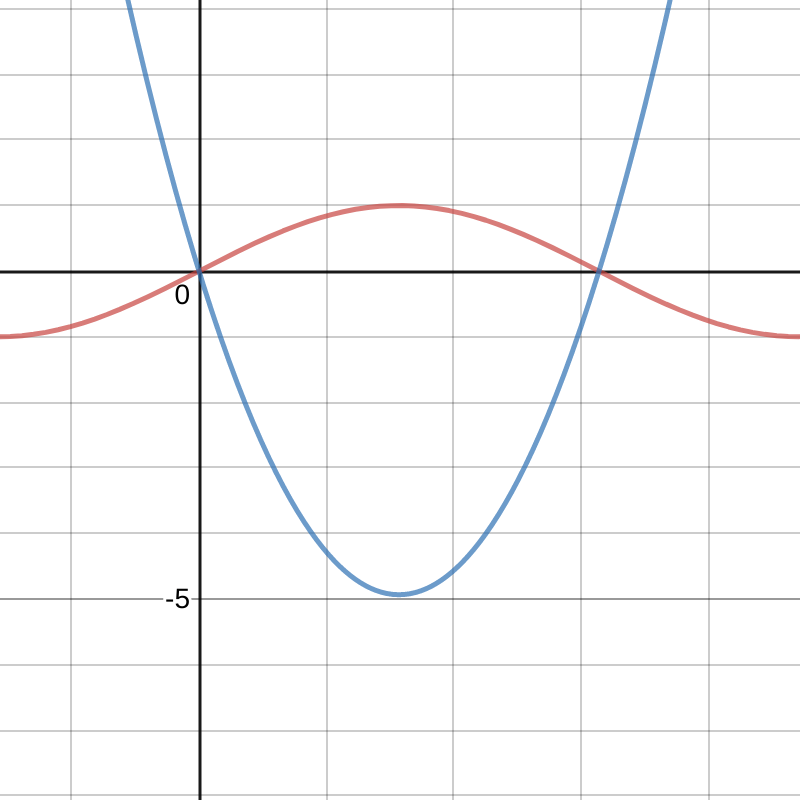
\includegraphics[width=0.6\linewidth]{graph}
			\end{center}
			
		\end{solution}
		
		\question Calcular $ \int_{-17\pi}^{17\pi} x^{2}\sin^{17}(3x)\cos^{3}(17x)\dif x $.
		
		\begin{solution}
			Pela propriedade aditiva das integrais, temos
			\[ \int_{-17\pi}^{17\pi} x^{2}\sin^{17}(3x)\cos^{3}(17x)\dif x = \int_{0}^{17\pi} x^{2}\sin^{17}(3x)\cos^{3}(17x)\dif x + \int_{-17\pi}^{0} x^{2}\sin^{17}(3x)\cos^{3}(17x)\dif x, \]
			e, por definição,
			\[ \int_{-17\pi}^{0} x^{2}\sin^{17}(3x)\cos^{3}(17x)\dif x = \int_{0}^{17\pi} (-x)^{2}\sin^{17}(-3x)\cos^{3}(-17x)\dif x. \]
			
			Sendo $ (-x)^{2}=x^{2} $, $ \cos x $ uma função par e $ \sin x $ uma função ímpar, temos
			\[ \int_{0}^{17\pi} (-x)^{2}\sin^{17}(-3x)\cos^{3}(-17x)\dif x = \int_{0}^{17\pi} x^{2}\del{-\sin(3x)}^{17}\cos^{3}(17x)\dif x \]
			e, portanto, a integral desejada é da forma
			\[ \int_{0}^{a}f(x)\dif x-\int_{0}^{a}f(x)\dif x \]
			que iguala zero.
		\end{solution}
		
		\question Seja $ \phi(x) = x - \floor{x}, x \in \mathbb{R} $.
		
		\begin{parts}
			\part Calcule $ T \in \mathbb{R} $ tal que $  \phi(x) \dif x = \sqrt{17}$.
			\part Tome $ a \in \mathbb{R} $ e calcule $ \lambda \in \mathbb{R} $ tal que $ \int_{a}^{a+\lambda} \phi(x) \dif x = \sqrt{2} $.
		\end{parts}
		
		\question Sejam $ n $ e $ m $ naturais não nulos. Calcule:
		\begin{parts}
			\part $ \int_{-\pi}^{\pi} \cos(n\,x)\sin(m\,x)\dif x $,
			
			\begin{solution}
				Tomando $ \alpha $ e $ \beta $ números arbitrários, temos
				\begin{align}
					&\dfrac{1}{2}\del{\sin(\alpha+\beta)+\sin(\alpha-\beta)}\nonumber\\
					&=\dfrac{1}{2}\del{\sin\alpha\cos\beta+\sin\beta\cos\alpha+\sin\alpha\cos\beta-\sin\beta\cos\alpha}\nonumber\\
					&=\sin\alpha\cos\beta,\label{eq:scsp}
				\end{align}
				que é conhecida como transformação de soma em produto.
				
				Tomando $ n=(a+b)/2 $ e $ m=(a-b)/2 $,\footnote{Note que $ a=n+m,b=n-m $.} para $ a,b $ arbitrários, temos, pela transformação de soma em produto:
				\[ \int_{-\pi}^{\pi} \cos(n\,x)\sin(m\,x)\dif x=\int_{-\pi}^{\pi}\dfrac{1}{2}\del{\sin(a\,x)+\sin(b\,x)} \dif x. \]
				O que nos dá o resultado
				\[ \dfrac{1}{2}\del{\eval{\del{-\dfrac{1}{a}\cos(a\,x)}}_{-\pi}^{\pi}+\eval{\del{-\dfrac{1}{b}\cos(b\,x)}}_{-\pi}^{\pi}}=-\dfrac{1}{2}\del{\dfrac{1}{a}\del{\cos (a\pi)-\cos(-a\pi)}+\dfrac{1}{b}\del{\cos (b\pi)-\cos(-b\pi)}} \]
				que iguala zero.
			\end{solution}
			
			\part $ \int_{-\pi}^{\pi} \cos(n\,x)\cos(m\,x)\dif x $ e $ \int_{-\pi}^{\pi}\sin(n\,x)\sin(m\,x)\dif x $, se $ n\neq m $,
			
			\begin{solution}
				Tomando $ \alpha $ e $ \beta $ números arbitrários, temos
				\begin{align}
					&\dfrac{1}{2}\del{\cos(\alpha+\beta)+\cos(\alpha-\beta)}\nonumber\\
					&=\dfrac{1}{2}\del{\cos\alpha\cos\beta-\sin\beta\sin\alpha+\cos\alpha\cos\beta+\sin\beta\sin\alpha}\nonumber\\
					&=\cos\alpha\cos\beta,\label{eq:ccsp}
				\end{align}
				e, também
				\begin{align}
					&\dfrac{1}{2}\del{\cos(\alpha-\beta)-\cos(\alpha+\beta)}\nonumber\\
					&=\dfrac{1}{2}\del{\cos\alpha\cos\beta+\sin\beta\sin\alpha-\cos\alpha\cos\beta+\sin\beta\sin\alpha}\nonumber\\
					&=\sin\alpha\sin\beta,\label{eq:sssp}
				\end{align}
			
				Tomando $ n=(a+b)/2 $ e $ m=(a-b)/2 $, para $ a,b $ arbitrários e aplicando \ref{eq:ccsp} na integral do produto dos cossenos, temos
				\[ \int_{-\pi}^{\pi} \cos(n\,x)\cos(m\,x)\dif x=\int_{-\pi}^{\pi} \dfrac{1}{2}\del{\cos(a\,x)+\cos(b\,x)}\dif x. \]
				O que nos dá o resultado
				\begin{align*}
					\dfrac{1}{2}\del{\eval{\del{\dfrac{1}{a}\sin(a\,x)}}_{-\pi}^{\pi}+\eval{\del{\dfrac{1}{b}\sin(b\,x)}}_{-\pi}^{\pi}}&=\\
					\dfrac{1}{2}\del{\dfrac{1}{a}\del{\sin (a\pi)-\sin(-a\pi)}+\dfrac{1}{b}\del{\sin (b\pi)-\sin(-b\pi)}}&=\\
					=&\dfrac{\sin (a\pi)}{a}+\dfrac{\sin (b\pi)}{b}
				\end{align*}
			
				Aplicando \ref{eq:sssp} na integral do produto dos senos, temos
				\[ \int_{-\pi}^{\pi} \sin(n\,x)\sin(m\,x)\dif x=\int_{-\pi}^{\pi} \dfrac{1}{2}\del{\cos(b\,x)-\cos(a\,x)}\dif x. \]
				O que nos dá o resultado
				\begin{align*}
					\dfrac{1}{2}\del{\eval{\del{\dfrac{1}{b}\sin(b\,x)}}_{-\pi}^{\pi}-\eval{\del{\dfrac{1}{a}\sin(a\,x)}}_{-\pi}^{\pi}}=&\\
					\dfrac{1}{2}\del{\dfrac{1}{b}\del{\sin (b\pi)-\sin(-b\pi)}-\dfrac{1}{a}\del{\sin (a\pi)-\sin(-a\pi)}}=&\\
					=&\dfrac{\sin (b\pi)}{b}-\dfrac{\sin (a\pi)}{a}.
				\end{align*}
				
			\end{solution}
			
			\part $ \int_{-\pi}^{\pi}\cos^{2}(n\,x)\dif x $ e $ \int_{-\pi}^{\pi}\sin^{2}(n\,x)\dif x $.
			
			\begin{solution}
				Basta notar que $ \cos^{2}(n\,x)=\cos(n\,x)\cos(m\,x) $ para $ n=m $ (idem para os senos). Dessa forma temos um caso particular da questão anterior, e, sendo $ n=a/2 $, temos
				\[ \int_{-\pi}^{\pi} \cos(n\,x)\cos(n\,x)\dif x=\int_{-\pi}^{\pi} \dfrac{1}{2}\cos(a\,x)\dif x \]
				o que nos dá o resultado
				\[ \dfrac{1}{2}\eval{\dfrac{1}{a}\sin(a\,x)}_{-\pi}^{\pi}=\dfrac{1}{a}\sin(a\,\pi), \]
				
				e
				\[ \int_{-\pi}^{\pi} \sin(n\,x)\sin(n\,x)\dif x=\int_{-\pi}^{\pi} -\dfrac{1}{2}\cos(a\,x)\dif x \]
				o que nos dá o resultado
				\[ -\dfrac{1}{2}\eval{\dfrac{1}{a}\sin(a\,x)}_{-\pi}^{\pi}=-\dfrac{1}{a}\sin(a\,\pi). \]
			\end{solution}
		\end{parts}
		
		\question Use o que foi visto na disciplina e calcule $ \sin\dfrac{\pi}{3} $.
		
		\begin{solution}
			Sabemos o cosseno de $ \pi $, dessa forma, encontrando o cosseno de arco triplo, podemos encontrar a resposta desejada, portanto:
			\begin{align*}
				\sin(3x)=\sin(2x+x)&=\sin 2x\cos x+\cos 2x\sin x\\
				&=\del{2\sin x\cos x}\cos x+(\cos^{2}x-\sin^{2}x)\sin x\\
				&=3\sin x\cos^{2}x-\sin^{3}x=3\sin x\del{1-\sin^{2}x}-\sin^{3}x\\
				&=3\sin x-4\sin^{3}x
				\implies\sin \pi&\sin\del{\pi/3}\del{3-4\sin^{2}\del{\pi/3}}=0,
			\end{align*}
			Como $ \sin(\pi/3)=0 $ é uma solução trivial, temos $ \sin^{2}(\pi/3)=3/4\implies\sin(\pi/3)=\pm\sqrt{3/4} $. Porém, como estamos analisando um ângulo no primeiro quadrante, temos que $\sin \pi/3\geqslant 0$, dessa forma: $ \sin (\pi/3)=\sqrt{3}/2 $.
			
		\end{solution}
		
		\question Seja $ f : [a, b] \to \mathbb{R} $ uma função integrável. Prove que $ \int_{a}^{b} f(x) \dif x = (b − a) \int_{0}^{1} f(a+(b−a)x)\dif x $ (use o que se viu na disciplina até aqui).
		
		\begin{solution}
			Essa demonstração segue trivialmente de uma expansão e translação da função:
			
			\begin{enumerate}
				\item Primeiro vamos expandir a função por um fator $ k $ (teorema 1.19):
				\[ \int_{a}^{b} f(x) \dif x=\dfrac{1}{k}\int_{k\,a}^{k\,b} f\del{\dfrac{x}{k}} \dif x, \]
				onde $ k=1/(b-a) $.
				\item Depois vamos transladar a função por um fator $ c $ (teorema 1.18):
				\[ \dfrac{1}{k}\int_{k\,a}^{k\,b} f\del{\dfrac{x}{k}} \dif x=\dfrac{1}{k}\int_{k\,a+c}^{k\,b+c} f\del{\dfrac{x-c}{k}} \dif x, \]
				onde $ c=-a/(b-a) $.
			\end{enumerate}
		
			Dessa forma, temos
			\[ (b-a)\int_{a/(b-a)-a/(b-a)}^{b/(b-a)-a/(b-a)} f\del{(b-a)\del{x+\dfrac{a}{(b-a)}}} \dif x=(b − a) \int_{0}^{1} f(a+(b−a)x)\dif x. \]
			
			\hfill\qedsymbol
		\end{solution}
		
		\question 
		\begin{parts}
			\part Seja $ f : [a, b] \to \mathbb{R} $ uma função integrável com $ f(x) \geqslant 0 $, para todo $ x \in [a, b] $. Defina $ A(x) = \int_{a}^{x} f(s)\dif s, x \in [a, b] $. Prove que $ A $ é integrável.
			
			\part Seja $ g : [a, b] \to R $ uma função integrável e defina $ G(x) = \int_{0}^{x} f(s)\dif s, x \in a [a, b] $. Prove que $ G $ é integrável.
		\end{parts}
	
		\question Sejam $ p > 0 $ e $ f : \mathbb{R} \to \mathbb{R} $ periódica de perı́odo $ p $ (isto é, $ f(x + p) = f(x) $, para todo $ x \in \mathbb{R} $) e integrável em todo intervalo $ [a, b] $ da reta. Mostre que, fazendo $ g(x) = \int_{0}^{x}f (t)\dif t $ e $ A = g(p/2) $,	tem–se:
		\begin{enumerate}
			\item $ g(x + p) − g(x) = g(p) $, para todo $ x \in \mathbb{R} $.
			
			\begin{solution}
				Tomando a diferença das integrais avaliadas, temos
				\begin{align*}
					g(x + p) − g(x) &= \int_{0}^{x+p}f (t)\dif t - \int_{0}^{x}f (t)\dif t\\
					\intertext{translacionando a primeira integral por $ -p $, temos}
					&= \int_{-p}^{x}f (t+p)\dif t - \int_{0}^{x}f (t)\dif t\\
					&=\int_{-p}^{0} f(t+p)\dif t+\int_{0}^{x}\underbrace{f (t+p)}_{=f(t)}\dif t - \int_{0}^{x}f (t)\dif t\\
					\intertext{translacionando a primeira integral por $ p $, temos}
					&=\int_{p}^{0} f(t)\dif t
				\end{align*}
			
				\hfill\qedsymbol
			\end{solution}
			
			\item Prove que $ g $ é periódica se, e só se, $ \int_{0}^{p} f (t)\dif t = 0 $.
			
			\begin{solution}
				Se $ g(x+p)-g(x)=g(p) $, segue que se $ g(p)=0 $, $ g(x+p)=g(x) $, que é a nossa definição de periodicidade. E se $ g(x+p)=g(x) $, temos, similarmente à letra (a):
				\begin{align*}
					\int_{0}^{x+p}f(t)\dif t&=\int_{0}^{x}f(t)\dif t\\
					\implies \int_{-p}^{x}f(t+p)\dif t&=\int_{0}^{x}f(t)\dif t\\
					\implies \int_{-p}^{0}f(t+p)\dif t+\int_{0}^{x}\underbrace{f(t+p)}_{=f(t)}\dif t&=\int_{0}^{x}f(t)\dif t\\
					\implies \int_{0}^{p}f(t)\dif t+\int_{0}^{x}f(t)\dif t&=\int_{0}^{x}f(t)\dif t\\
					\implies \int_{0}^{p}f(t)\dif t&=0
				\end{align*}
			
				\hfill\qedsymbol
			\end{solution}
			
			\item Suponha que $ f $ é uma função par e calcule $ g(n\,p/2) $ em função de $ A $, para $ n \in \mathbb{N} $ (sugestão: considere inicialmente o caso $ n = 2 $ e resolva-o, o resto deve ser simples).
			
			\begin{solution}
				Tomando $ n=2 $, temos
				\[ g(2p/2)=g(p)=\int_{0}^{p}f(t)\dif t, \]
				translacionando por $ -p/2 $, temos, pela paridade da função
				\[ \int_{-p/2}^{p/2}f(t+p/2)\dif t=2\int_{0}^{p/2}f(t+p/2)\dif t \]
				transladando por $ p/2 $, temos
				\[ 2\int_{p/2}^{p}f(t)\dif t=2\int_{0}^{p}f(t)\dif t-2\int_{0}^{p/2}f(t)\dif t. \]
				
				Ou seja, vale que $ g(2p/2)=g(p)=2g(p)-2A\iff g(p)=2A $.
				
				Assumindo $ g(n\,p/2)=n\,A $, vamos provar que $ g\del{(n+1)p/2}=\del{n+1}A $:
				\begin{align*}
					\int_{0}^{n\,p/2}f(t)\dif t&=n\int_{0}^{p/2}f(t)\dif t\\
					\int_{0}^{n\,p/2}f(t)\dif t+\int_{0}^{p/2}f(t)\dif t&=n\int_{0}^{p/2}f(t)\dif t+\int_{0}^{p/2}f(t)\dif t\\
					\int_{0}^{n\,p/2}f(t)\dif t+\int_{n\,p/2}^{n\,p/2+p/2}f(t-n\,p/2)\dif t&=\del{n+1}\int_{0}^{p/2}f(t)\dif t.
				\end{align*}
				
				Avaliando a paridade de $ \int_{n\,p/2}^{n\,p/2+p/2}f(t-n\,p/2)\dif t $, temos
				\begin{itemize}
					\item Para $ n=2m $ (par), temos:
					\[ \int_{n\,p/2}^{n\,p/2+p/2}f(t-2m\,p/2)\dif t=\int_{n\,p/2}^{n\,p/2+p/2}f(t)\dif t, \]
					ou seja
					\[ \int_{0}^{n\,p/2}f(t)\dif t+\int_{n\,p/2}^{n\,p/2+p/2}f(t)\dif t=\int_{0}^{(n+1)p/2}f(t)\dif t=\del{n+1}\int_{0}^{p/2}f(t)\dif t. \]
					\hfill\qedsymbol
					\item Para $ n=2m-1 $ (ímpar) eu não sei.
				\end{itemize}
			\end{solution}
		\end{enumerate}
	
		\question Sejam $ f $ e $ g $ funções definidas no intervalo $ [0, 1] $ tomando valores em $ \mathbb{R} $, ambas limitadas. Suponha que $ f (x) $ é integrável.
		\begin{parts}
			\part Suponha que $ f (x) = g(x) $, para todo $ x \in [0, 1] \backslash F $ onde $ F \subset [0, 1] $ é um conjunto finito. Prove que $ g(x) $ é integrável e $ \int_{0}^{1} g(x)\dif x = \int_{0}^{1} f (x)\dif x $.
			
			\part Suponha que $ f (x) = g(x) $, se $ x \in [0, 1] \backslash \set{ 1/n , n \in \mathbb{N}^{\star} } $. Prove que $ g(x) $ é integrável e $ \int_{0}^{1} g(x)\dif x = \int_{0}^{1} f (x)\dif x $.
		\end{parts}
		
		
		
%		\begin{parts}
%			\part 
%			
%			\begin{solution}
%				
%			\end{solution}
%		
%			\part 
%			\begin{solution}
%				
%			\end{solution}
%			
%			\part 
%			\begin{solution}
%				
%				\begin{lemma}\label{lemma:lem1}
%					Dado $ a $ real, $ a>0\iff a^{-1}>0 $.
%				\end{lemma}
%				
%				\begin{proof}
%					Seja $ b=a^{-1}\cdot a^{-1}=(a^{-1})^{2} $, pelo teorema 1.20 temos que $ b>0 $ e, dessa forma, $ a\cdot b=a(a^{-1}\cdot a^{-1})=(a\cdot a^{-1})a^{-1}=a^{-1} $ que também deve pertencer a $ \mathbb{R}^{+} $ (axioma 7). (Note que automaticamente vale a recíproca)
%				\end{proof}
%				
%				\begin{lemma}\label{lemma:lem2}
%					Dados $ a,b\in\mathbb{R}^{+} $ tais que $ 0<a<b $, teremos que seus inversos obedecem $ 0<b^{-1}<a^{-1} $.
%				\end{lemma}
%				
%				\begin{proof}
%					Sendo $ b>a $ vale que $ b^{-1}\cdot b = 1 > b^{-1}\cdot a $, e disso, temos $ a^{-1}\cdot 1 > (a^{-1}\cdot a)\cdot b^{-1}=b^{-1} $. E pelo lema \ref{lemma:lem1}, temos que $ 0<b^{-1}<a^{-1} $.
%				\end{proof}
%				
%				\begin{lemma}
%					Dado um real positivo $ x $, vale que, (a) se $ x>1 $, temos $ 0<x^{-1}<x $ e (b) se $ 0<x<1 $, temos $ 0<x<x^{-1} $.
%				\end{lemma}
%				
%				\begin{proof}
%					Pelo axioma 6, o inverso de 1 é ele mesmo (trivial), dessa forma, pelo teorema 1.21, no primeiro caso (a) do lema, temos $ 0<1<x $, e pelo lema \ref{lemma:lem2} vale que $ 0<x^{-1}<1<x $ e, automaticamente, vale que $ 0<x^{-1}<x $. Para o segundo caso (b) temos uma demonstração equivalente ($ 0<x<1\overset{\textup{\small lema \ref{lemma:lem2}}}{\implies}0<x<1<x^{-1} $).
%				\end{proof}
%			
%				Dessa forma, segue que, para $ a>1,a\in A $, temos $ 0<a^{-1}<1<a $, de tal forma que, para $ a_2>a_1>1 $, os respectivos $ b_1=a_1^{-1} $ e $ b_2=a_2^{-1} $ ficam na ordem $ b_2>b_1>1>b_1^{-1}>b_2^{-1}>0 $, e para $ a_n $, com $ n $ grande o suficiente, conseguimos um $ b $ tão perto de zero quanto se queira (definitivamente não é um supremo, mas pode ser um ínfimo).
%				
%				Para $ a=1 $ segue que $ b=1 $, porém, para $ 0<a<1 $ temos o comportamento inverso do parágrafo anterior. Sendo $ 0<a<1<a^{-1} $, dados $ 0<a_2<a_1<1 $, teremos $ 0<a_2<a_1<1<a_1^{-1}<a_2^{-1} $, e a sequência de elementos de $ B $ poderá ser tão grande quanto menor seja $ a\in A $. Se $ \inf A>0 $, existe somente um $ a_m\in A $ tal que $ \inf A=a_m $, e como $ 0<a_m<a_n $ para qualquer $ a_n\in A $, $ b_m=a_m^{-1} $ deve ser o maior $ b\in B $ (i.e. seu supremo).
%				
%				Para $ \inf A=0 $ não existe $ a\in A $ cumprindo o papel de $ a_m $, e não deve haver majorante para $ B $, pois sempre haverá um $ 0<k<a_n $ tal que $ k^{-1}>a_n^{-1} $. 
%				
%				\hfill\qedsymbol
%			\end{solution}
			
%			\part 
%			\begin{solution}
%			
%			\end{solution}
%		\end{parts}
		
		
	\end{questions}
\end{document}